\section{Uppgift 7}\label{sec:uppg07}

\subsection{Instruktioner}
\begin{verbatim}
7. Ett heltal är ett primtal om det bara är delbart med 1 och sig självt.
   Exempelvis så är 2, 3, 5 och 7 primtal, men 4, 6, 8 och 9 är ej primtal.
   Skriv ett program som kontrollerar och skriver ut om ett tal är primtal
   eller ej. Den som kör programmet ska skriva in talet.
   Tips: använd modulus-operatorn %.
\end{verbatim}


\subsection{Lösning}

\subsubsection{Källkod}
\javacode{src/main/Lab2Uppg07.java}
\caption{Lab2Uppg07.java}
\label{src:uppg07}


\subsubsection{Skärmdump}
\begin{figure}[htbp]
    \centering
        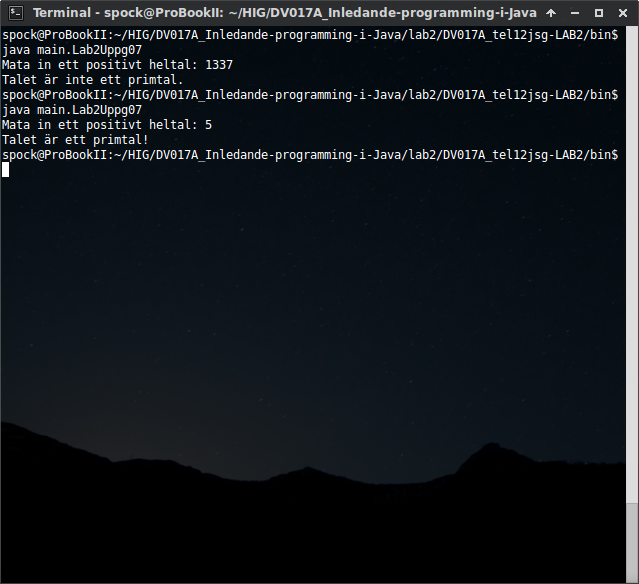
\includegraphics[width=\linewidth]{img/07.png}
    \caption{Körning av koden till Uppgift~\ref{sec:uppg07}}
    \label{fig:uppg07-screenshot}
\end{figure}

